\chapter{Формирование и анализ моделей}
\section{Создание моделей}
На основе обучающей выборки, были построены две модели линейной регрессии\cite{wapnick2009}: базовая (Drinks\_per\_week от Party\_Hours\_per\_week + Gender) и расширенная (Drinks\_per\_week от Party\_Hours\_per\_week + Gender + Home\_Town). Программный код представлен в листинге \ref{lst:models}.
\lstinputlisting[language=R,caption=Создание моделей в R,label=lst:models]{listings/models.R}

\begin{table}[h]
	\centering
	\caption{Сводная информация по первой модели: \texttt{Drinks\_per\_week} $\sim$ \texttt{Party\_Hours\_per\_week} + \texttt{Gender}}
	\begin{tabular}{lrrrr}
		\hline
		\textbf{Коэффициент} & \textbf{Оценка} & \textbf{Ст. ошибка} & \textbf{t-стат.} & \textbf{p-значение} \\
		\hline
		(Intercept)             & 1.63  & 0.37 & 4.39  & 1.27e-06$^{***}$ \\
		Party\_Hours\_per\_week & 1.14  & 0.03 & 34.31 & $<$2e-16$^{***}$ \\
		Gender1                 & -2.25 & 0.39 & -5.73 & 1.34e-08$^{***}$ \\
		\hline
	\end{tabular}
	\vspace{0.5em}
	
	\textbf{Остатки:} \\
	Минимум: -46.40 \quad 1 кв.: -2.78 \quad Медиана: -0.511 \quad 3 кв.: 1.19 \quad Максимум: 43.36
	
	\vspace{0.5em}
	\textbf{Качество модели:} \\
	Стандартная ошибка остатков: 5.98 при 1019 степенях свободы \\
	Множественный $R^2$: 0.54 \quad Скорректированный $R^2$: 0.55 \\
	F-статистика: 614.3 при 2 и 1019 СС \quad p-значение: $<$2.2e-16
	\label{tab:m1}
\end{table}

\begin{table}[h]
	\centering
	\caption{Сводная информация по второй модели: \texttt{Drinks\_per\_week} $\sim$ \texttt{Party\_Hours\_per\_week} + \texttt{Gender} + \texttt{Home\_Town}}
	\begin{tabular}{lrrrr}
		\hline
		\textbf{Коэффициент} & \textbf{Оценка} & \textbf{Ст. ошибка} & \textbf{t-стат.} & \textbf{p-значение} \\
		\hline
		(Intercept)             & 1.85  & 0.45 & 4.09  & 4.56e-05$^{***}$ \\
		Party\_Hours\_per\_week & 1.15  & 0.03 & 34.28 & $<$2e-16$^{***}$ \\
		Gender1                 & -2.23 & 0.40 & -5.63 & 2.38e-08$^{***}$ \\
		Home\_Town              & -0.36 & 0.41 & -0.86 & 0.39 \\
		\hline
	\end{tabular}
	\vspace{0.5em}
	
	\textbf{Остатки:} \\
	Минимум: -46.35 \quad 1 кв.: -2.65 \quad Медиана: -0.420 \quad 3 кв.: 1.25 \quad Максимум: 48.50
	
	\vspace{0.5em}
	\textbf{Качество модели:} \\
	Стандартная ошибка остатков: 5.97 при 1018 степенях свободы \\
	Множественный $R^2$: 0.55 \quad Скорректированный $R^2$: 0.55 \\
	F-статистика: 409.7 при 3 и 1018 СС \quad p-значение: $<$2.2e-16
	\label{tab:m2}
\end{table}

Сводная информация по построенным моделям представлена в таблицах~\ref{tab:m1}--\ref{tab:m2}. Как видно, включение переменной \texttt{Home\_Town} не является статистически значимым (p = 0.39). Однако изменилось значение свободного члена (Intercept), что указывает на возможное влияние города происхождения на базовый уровень потребления.

\section{Оценка моделей}

Проведём оценку обеих моделей на тестовой выборке (листинг~\ref{lst:fstat}).
\lstinputlisting[language=R,caption=Вычисление F-статистики,label=lst:fstat]{listings/Fstatistic.R}

Для первой модели начение F-статистики \cite{wapnick2009} равно 2066.952. Для второй - 2097.124.

Значения F-статистики намного больше 1, что указывает на то, что обе модели в целом значимы.
Вторая модель имеет немного более высокую F-статистику (2097.124 против 2066.952), что может говорить о её чуть лучшей объясняющей способности.

\section{Графики моделей}

Построим графики обеих моделей (рисунок~\ref{fig:models}, код представлен в приложении \ref{ch:rgph1}).


\begin{figure}[h]
	\centering
	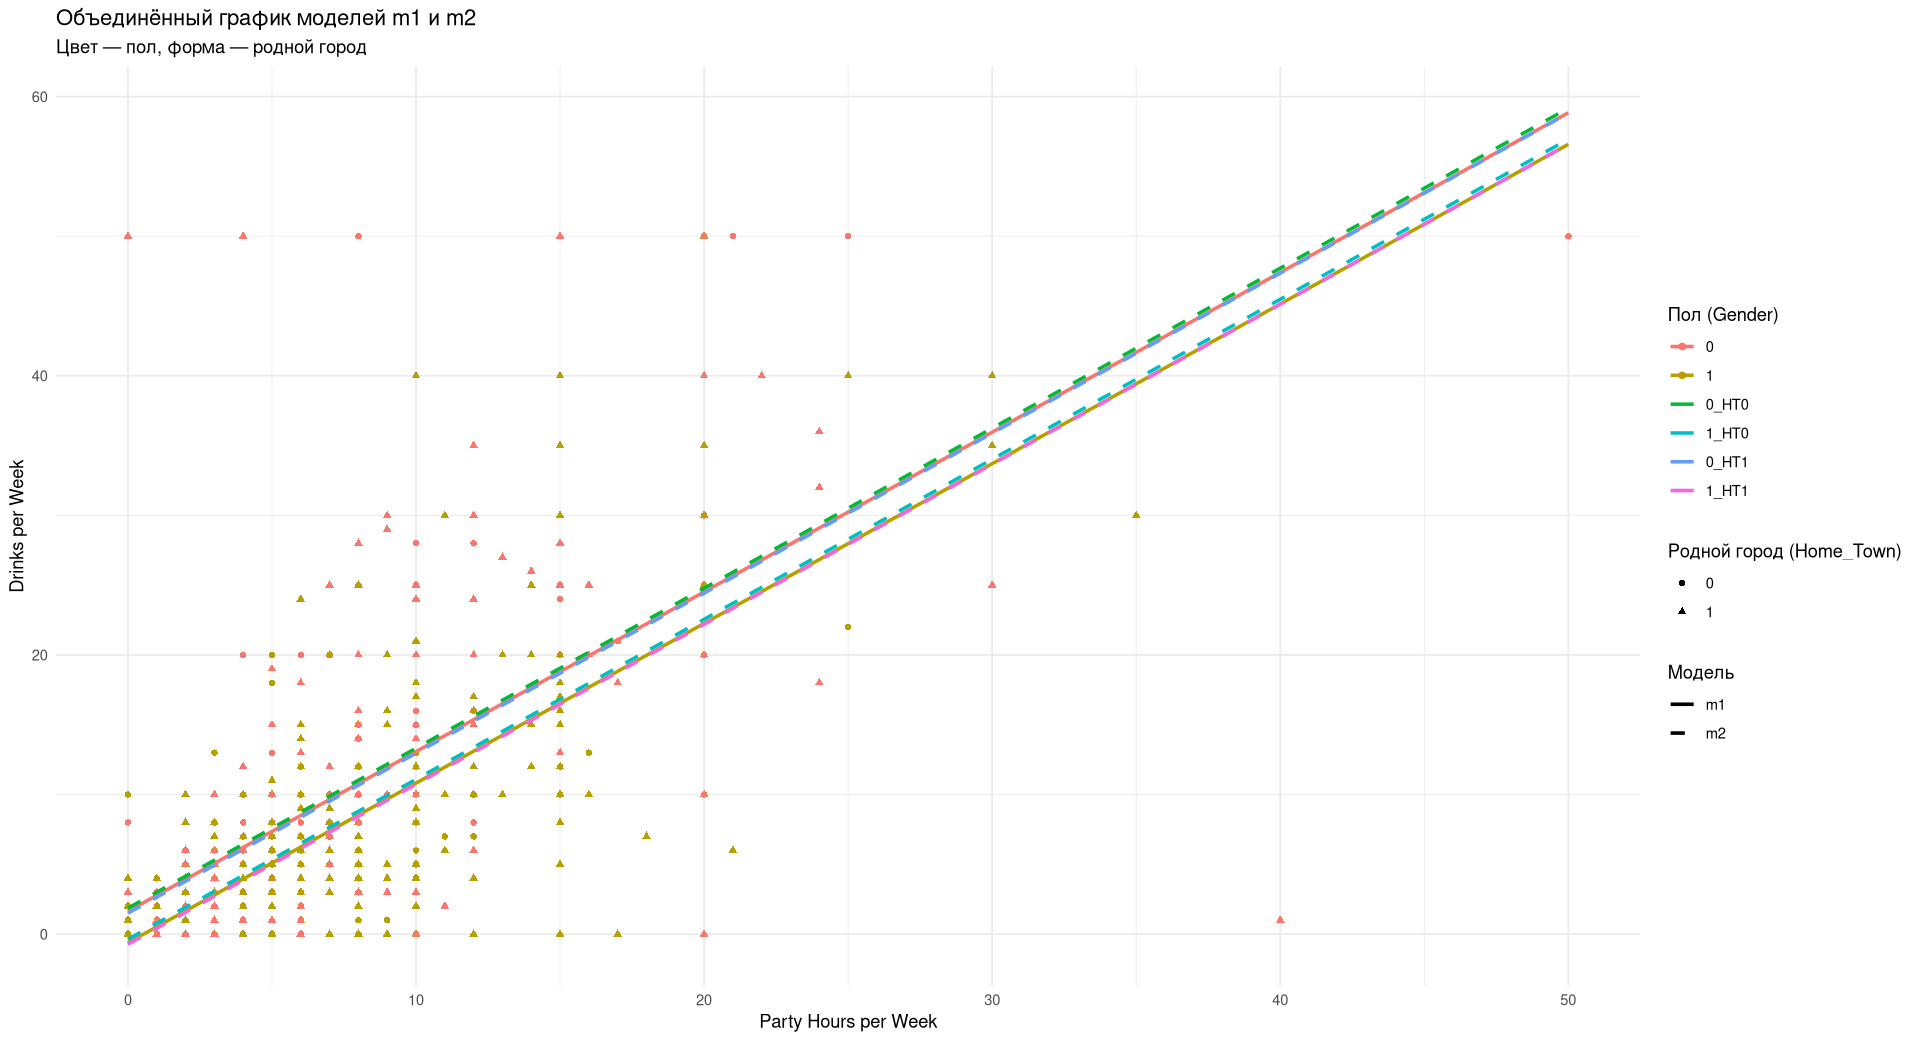
\includegraphics[height=0.6\textwidth]{imgs/models.png}
	\caption{Графики регрессионных моделей}
	\label{fig:models}
\end{figure}

На рисунке~\ref{fig:models} видно, что обе модели дают параллельные прямые для каждого пола. Это объясняется одинаковым коэффициентом переменной \texttt{Party\_Hours\_per\_week}, который отражает вклад вечернего поведения вне зависимости от пола.




\section{Доверительные и предиктивные интервалы}
\subsection*{Расчёт новых данных}
Рассчитаем предсказания для значений переменной \texttt{Party\_Hours\_per\_week}, увеличенных на 5\%, 10\% и 15\% от её максимума, для обоих полов, используя первую модель (таб. \ref{tab:pred_intervals}, листинг~ \ref{lst:newdata}).

\lstinputlisting[language=R,caption=Предсказания новых значений,label=lst:newdata]{listings/newdata.R}

\begin{table}[ht]
	\centering
	\caption{Предсказания и интервалы для переменных}
	\begin{tabular}{|l|r|r|r|r|r|r|r|r|}
		\hline
		Party\_Hours & Gender & Fit & Lwr & Upr & Pred\_Lwr & Pred\_Upr \\
		\hline
		52.5 & 0 & 61.70 & 58.58 & 64.82 & 49.55 & 73.86 \\
		55.0 & 0 & 64.57 & 61.28 & 67.85 & 52.37 & 76.76 \\
		57.5 & 0 & 67.43 & 63.98 & 70.87 & 55.19 & 79.66 \\
		52.5 & 1 & 59.45 & 56.32 & 62.57 & 47.29 & 71.60 \\
		55.0 & 1 & 62.31 & 59.02 & 65.59 & 50.11 & 74.50 \\
		57.5 & 1 & 65.17 & 61.72 & 68.61 & 52.93 & 77.41 \\
		\hline
	\end{tabular}
	\label{tab:pred_intervals}
\end{table}

Построим доверительные и предиктивные интервалы\cite{wapnick2009} на всём промежутке (рисунок~\ref{fig:intervals}, код представлен в приложении \ref{ch:rgph2}).

\begin{figure}[h]
	\centering
	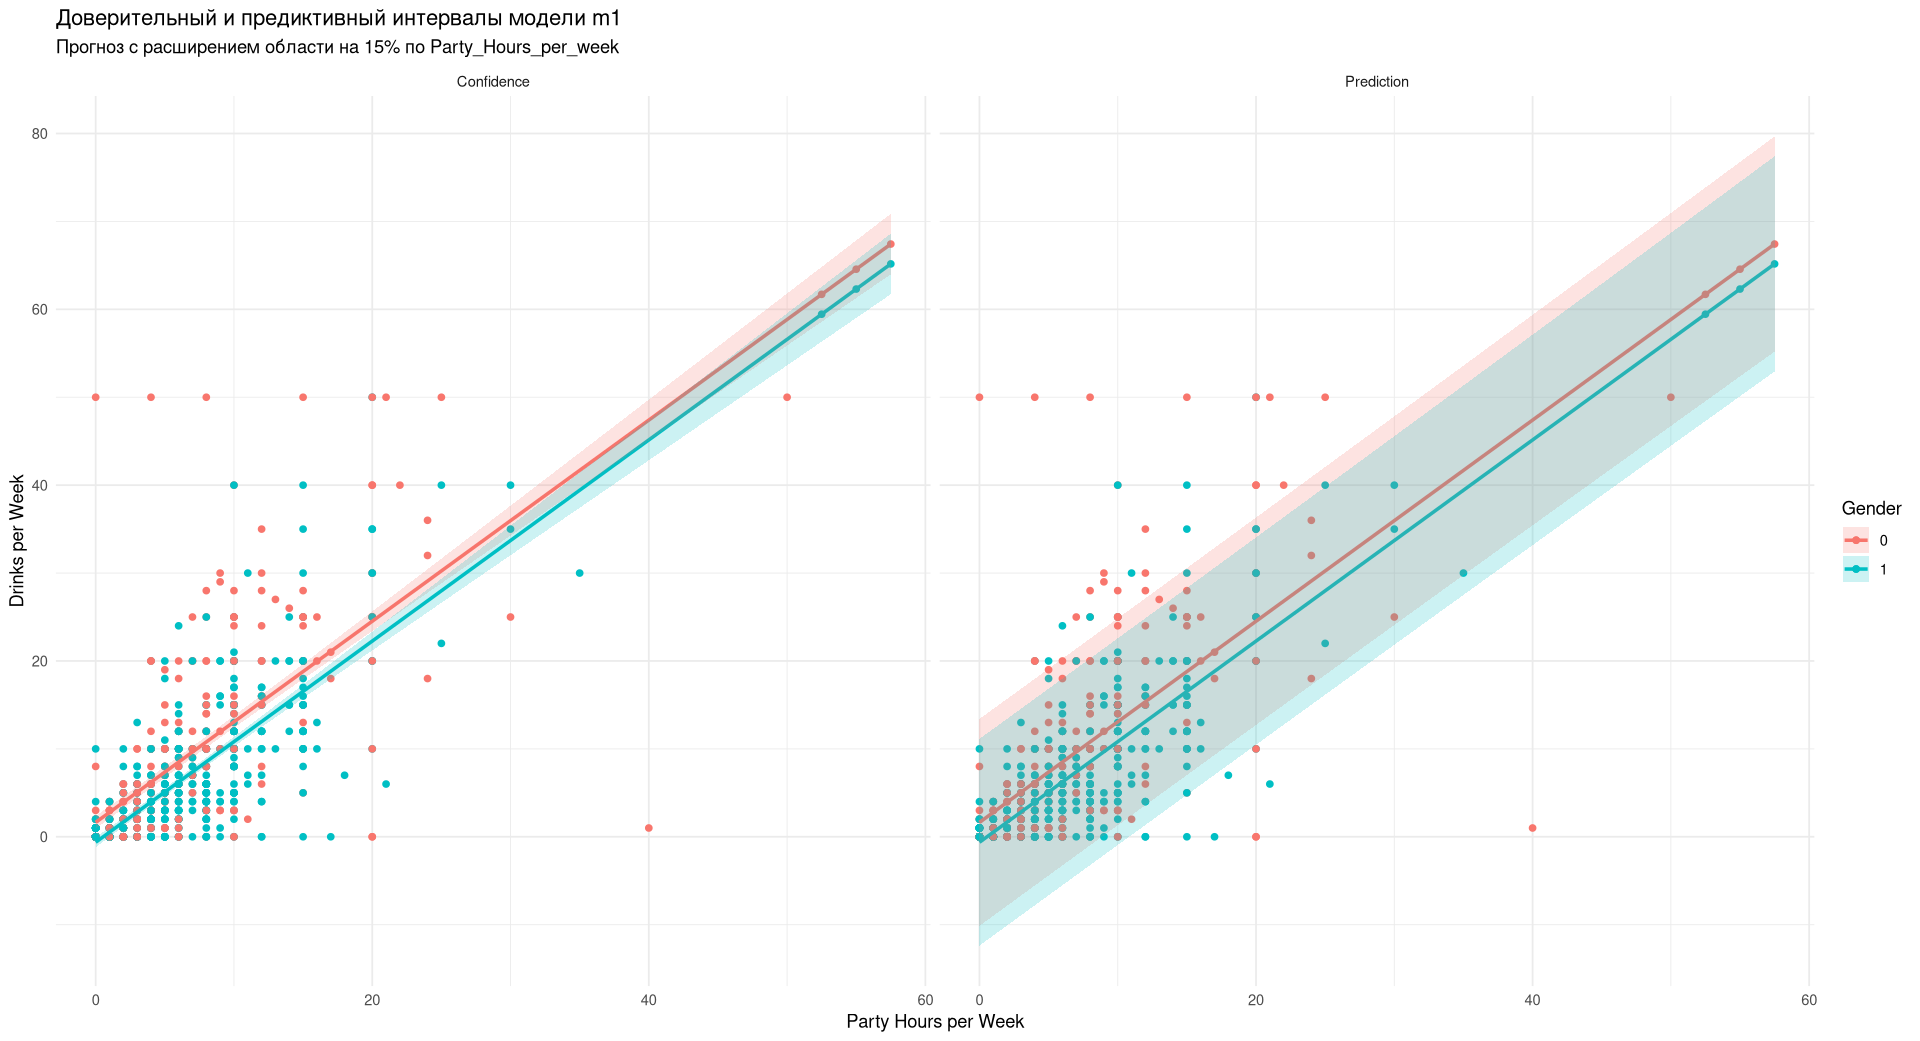
\includegraphics[height=0.6\textwidth]{imgs/intervals.png}
	\caption{Графики доверительных и предиктивных интервалов модели (на фоне точки тестовой выборки. Справа сверху шесть точек - новые предсказание +5-15\% от максимального значения всего датасета)}
	\label{fig:intervals}
\end{figure}

\subsection*{Доверительные интервалы (Confidence)}
Доверительные интервалы отображают неопределённость оценки среднего значения зависимой переменной при фиксированном значении независимой переменной. Видно, что интервалы более узкие в центральной части, где плотность наблюдений выше, и расширяются к краям, что типично при экстраполяции.

\subsection*{Предиктивные интервалы (Prediction)}
Предиктивные интервалы шире, так как учитывают не только ошибку оценки среднего, но и вариацию индивидуальных значений. Это позволяет:
\begin{itemize}
	\item Адекватно отображать разброс реальных наблюдений вокруг линии регрессии.
	\item Учесть существенно большую неопределённость при попытке предсказать индивидуальное поведение.
\end{itemize}

\subsection*{Область экстраполяции}
Интервалы построены с учётом расширения по оси \texttt{Party\_Hours\_per\_week} на 15\%, что наглядно демонстрирует:
\begin{itemize}
	\item Резкое расширение обоих типов интервалов за пределами основной области наблюдений.
	\item Повышенную неопределённость прогнозов вне обучающего диапазона данных.
\end{itemize}

\section*{Выводы}
\begin{itemize}
	\item Модель демонстрирует адекватную уверенность в оценке среднего, но справедливо расширяет предиктивные интервалы, что указывает на реалистичную оценку неопределённости.
	\item Наблюдаемое различие между полами при сохранении общей тенденции подтверждает обоснованность стратификации по полу.
\end{itemize}
